% Actual viewer capture and separately measured renderer diagnostics.
\section{Sweep Replay and Rendering Evidence}
\label{sec:c}

\begin{figure}[!htbp]
\centering
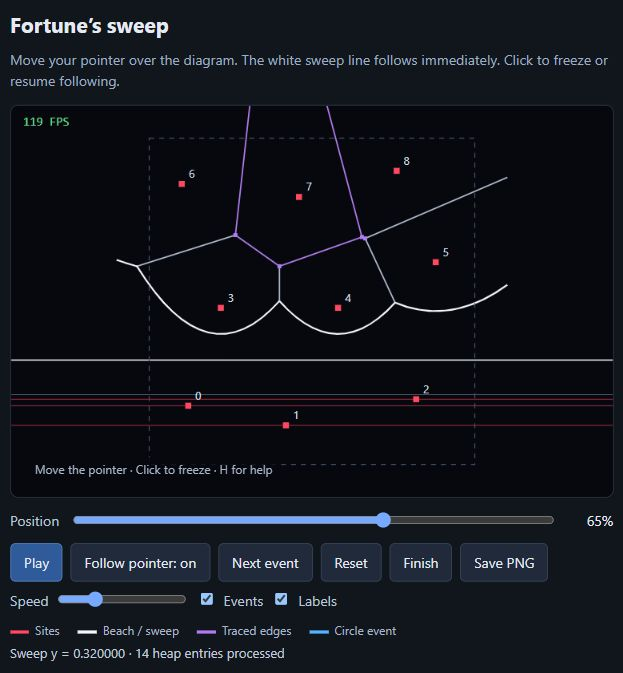
\includegraphics[width=0.83\linewidth,height=0.62\textheight,keepaspectratio]{canvas-preview.jpg}
\caption[Pointer-controlled Canvas sweep replay.]{Actual browser capture of the integrated viewer. Red squares are sites; white curves and the horizontal line are the beach line and directrix. Purple segments are traced edges. Event markers and controls expose the recorded Python event sequence.}
\label{fig:canvas-replay}
\end{figure}

Run \code{run.bat --animate --input examples\textbackslash sites.txt}. Hover to move the sweep line, click to freeze or resume following, or use Play and Next event. The exported HTML works offline. \path{docs/animation.md} describes controls, the collinear special case and the history limit.

\clearpage
\subsection{Rendering Bottleneck and Verification}

The first Matplotlib replay rebuilt axes, artists and interface text on every frame. A 50-site off-screen redraw took a median 234.36 ms, while event-model advancement took about 0.007 ms. Persistent artists, background caching and time-based playback improved the native Tk version to about 44.5 timer updates per second. The owner still found pointer interaction insufficiently fluid. The final viewer therefore records event facts once and draws them directly in browser Canvas.

\begin{table}[!htbp]
\centering
\caption{Observed browser rendering diagnostics, separate from construction.}
\label{tab:canvas-performance}
\begin{tabularx}{\linewidth}{@{}rXX@{}}
\toprule
\textbf{Sites} & \textbf{Rolling RAF rate} & \textbf{Median draw time} \\
\midrule
50 & 120.0 Hz & 1.4 ms \\
200 & 120.0 Hz & 2.4 ms \\
\bottomrule
\end{tabularx}
\end{table}

Measurements came from the visible in-app browser at 602 by 375 CSS pixels, with a 752 by 469 backing canvas. The rate measures rolling \code{requestAnimationFrame} callbacks, not physical display scanout; draw time covers recent Canvas work. These observations do not guarantee a frame rate on other displays or machines. Browser console checks reported no errors. Position changes, playback and Save PNG were exercised; the original downloaded image is \path{evidence/canvas-export.png}. Raw diagnostics are retained in \path{results/animation-preview/render-browser.json}.

The revised viewer uses the same Python event handlers as batch construction, but its stored arc orders can occupy $O(n^2)$ space. A 200-site limit keeps this educational trade-off explicit. Core construction creates no replay history. The owner approved the viewer's appearance and authorized main-branch integration on 18 November 2026. That approval does not substitute for the owner's narrated explanation of the algorithm.

Replay tests compare every snapshot with a separately run Python sweep and verify independent checkpoints. Two Node-based checks compare drawing geometry with Python in 100 cases and exercise pointer movement without a pressed button; they explicitly skip without Node. Installed-asset and browser checks cover offline export, positioning, playback and PNG download. Node is unnecessary to run the viewer.
